% \chapter{Design and implementation}

% This chapter may be called something else\ldots but in general the
% idea is that you have one (or a few) ``meat'' chapters which describe
% the work you did in technical detail.

% \chapter{Measuring Python's performance}
% \label{chap:understanding-compiler-performance}


\chapter{Understanding compiler performance}
\label{chap:understanding-compiler-performance}

% \textit{
% \textbf{TODO:}
% \begin{enumerate}
%     \item What performance do we care about (compilation time rather than performance of generated binary)?
%     \item Why do we care about (compilation time) performance?
%     \item What question(s) are we trying to answer?
%     \begin{enumerate}
%         \item How does xDSL compare to MLIR, particularly in relation to dynamism of workloads/language runtimes?
%         \item What are bottlenecks in xDSL which we could mitigate in the next chapter?
%     \end{enumerate}
%     \item How did we go about answering them?
% \end{enumerate}
% }

% \section{Methodology}
% \label{sec:methodology}

% \textit{
% \textbf{TODO:}
% \begin{enumerate}
%     \item What techniques did we use?
%     \item Detailed description of the experimental approach, for replicability and to convince readers of rigour.
%     \item Further benefits of experiments, such as performance regression infrastructure and empirically driven optimisation
% \end{enumerate}
% }

\section{Micro-benchmarking}
\label{sec:ubenchmark}

% Hook
Micro-benchmarking refers measuring the performance of fast, granular, and isolated segments of code.
% It contrasts traditional benchmarking approaches which instead examine the performance of larger code segments, typically representative of a real-world workload.
% Argument
The term was coined by Saavedra et al. in their 1995 paper \cite{saavedraPerformanceCharacterizationOptimizing1995} ``Performance Characterization of Optimizing Compilers'', suggesting we are in good company in our application of micro-benchmarking approaches to this problem domain.
Micro-benchmarks have many desirable properties. Since they run quickly, they can cheaply be repeated for statistical confidence.
Furthermore, their fine granularity makes them tractable to reason about -- providing useful information to optimise the component of the system they measure.
However, a key difficulty of micro-benchmarking is ensuring its alignment with overall system performance. For example, the selection of code paths for micro-benchmarking may introduce bias, making them less representative. In addition to this, their results may be inflated as a consequence of warmed caches and JIT optimisation across repeats, which would not occur during normal operation.
% Link
Micro-benchmarking is a useful tool for deeply understanding the performance of software, but must be used carefully to ensure the validity of its results.

%% Now the mlir community already disagree (cannot find source for this feeling, so elide), leading to talk
% Hook
At the 2024 European LLVM Developers' Meeting, Mehdi Amini and Jeff Nui
presented their keynote talk ``How Slow is MLIR?'' \cite{aminiHowSlowMLIR2024}.
% Argument
In this talk, they presented micro-benchmarks for key operations in the MLIR compiler, such as traversing the IR and creating operations. The micro-benchmarks were used to inform the optimisation of MLIR's data structures and for comparison with traditional LLVM-based compilers. The implementation of the micro-benchmarks allude to an underlying design goal in MLIR by their measurement of asymptotic scaling properties\footnote{\url{https://github.com/joker-eph/llvm-project/blob/6773f827b9ee8055063fcf6b2c6fcdc7f4f579d2/mlir/unittests/Benchmarks/Cloning.cpp\#L66}}. This design goal is asymptotically optimal performance for its underlying data structures. However, such data structures often incur constant-time penalties. This causes overhead for small workloads, where, unlike the asymptotic case, the cost is not amortised.
As such, micro-benchmarks may not be representative of the system's overall performance, revealing possibility for the optimisation of code co-designed using them.
% Link
Despite this, they can still provide useful insight into MLIR's performance characteristics. 

We implement micro-benchmark workloads for the xDSL equivalent to those for MLIR presented in the keynote. % and hot paths identified in constant folding workloads.
We then compare the results of these benchmarks between xDSL and MLIR, giving insights into their relative performance. We further leverage profiling tools to examine the call stacks of the two implementations. This allows us to distinguish between the cost incurred by the language runtime, and the cost incurred by the algorithmic approach of the implementation.





\subsection{Methodology}
\label{ssec:ubenchmark-methodology}

\subsubsection{Micro-benchmarking infrastructure}
\label{sssec:ubenchmark-methodology-infra}

% Link
% Micro-benchmark results are sensitive to machine noise due to their short lengthm
Due to their short length, micro-benchmark results are sensitive to machine noise and overhead incurred by their measurement instrumentation. As such, care must be taken constructing the methodology for these experiments.
% Argument
To minimise the impact of machine noise, experiments are repeated and averaged, with uncertainty calculated as their standard deviation. In addition to this, other mechanisms increase the variance of results.
Python triggers a full garbage collection when the number of new objects exceeds $25\%$ of the existing objects, adding a slow but infrequent overhead. To mitigate this, we manually invoke a full collection before each measurement. This guarantees ensures that collection is repeatable, but does not hide overhead incurred in real-world applications
% TODO: Add more
% Hook
Having constructed reliable infrastructure to run micro-benchmarks in Python, the next step in the methodology is to write implementations which are directly comparable to the existing MLIR versions. This is necessary to be able to draw conclusions about the differences between the Python and C++ runtimes for compiler framework workloads.

% Rubric about what machines, python/clang versions/... are being used
Furthermore, both the MLIR and xDSL microbenchmarks were run locally on the same experimental machine, whose hardware and software configuration is described in \autoref{tab:ubenchmark-experimental-config}. For all micro-benchmarks, the functions under test were measured $2^{15}$ times, reporting the mean value with an uncertainty given by the standard deviation.

\begin{table}[H]
  \caption{Experimental configuration used for micro-benchmarking.}
  % Note: this will be re-run on an AWS box soon
  \label{tab:ubenchmark-experimental-config}
  \centering
  \begin{tabular}{lll}
    \toprule
    \textbf{Configurable} & \textbf{Configuration} \\
    \midrule
    \textit{xDSL commit SHA} & \texttt{0eda7fe} \\
    \textit{MLIR commit SHA} & \texttt{6516ae4} \\
    \midrule
    \textit{Python interpreter} & CPython 3.12.9 \\
    \textit{C++ compiler} & clang 18.1.8 \\
    \textit{CMake version} & 3.31.3 \\
    \textit{Ninja version} & 1.12.1 \\
    \textit{Operating system} & macOS Sequoia 15.4.1 \\
    \midrule
    % \textit{Clock frequency [GHz]} & \\
    \textit{CPU} & Apple M3 \\
    \textit{RAM [GB]} & 16 \\
    \bottomrule
  \end{tabular}
\end{table}

\subsubsection{Micro-benchmarking implementation}
\label{sssec:ubenchmark-methodology-impl}

%% Finding and building the MLIR microbenchmarks
% Hook
Unfortunately, the implementation and build instructions for the ``How Slow is MLIR?'' micro-benchmarks were not published with the talk.
% Argument (too informal?)
However, their source code can be found on a branch of the presenter's fork of LLVM\footnote{\url{https://github.com/joker-eph/llvm-project/tree/benchmarks}}. We provide a copy of this source code and instructions for running the benchmarks\footnote{\url{https://github.com/EdmundGoodman/llvm-project-benchmarks}} to enhance the replicability of our results and facilitate further performance experiments.
% Link
This source code can then be used to construct comparable micro-benchmarks in Python.

% Design of our microbenchmarks
% Hook
A key design goal of our micro-benchmarks for xDSL is parity with those provided for MLIR, ensuring the validity their direct comparison. As such, their implementation was derived from the MLIR benchmarks, matching test data and function invocations as closely as possible.
% Argument







\subsection{Operation trait checks}
\label{ssec:ubenchmark-trait-checks}

% Two goals in the narrative here:
% - Introduce the difference between implementation and language, and approaches to mitigate this
% - Introduce dynamism as a common occurence, and understand why it is slow

% Hook
MLIR and xDSL both provide methods to check whether operations have traits.
% Argument
These methods are used very frequently, forming the basis of many tasks. For example, when pattern rewriting over a block of IR, the traits of the block's constituent operations are commonly used by the matching engine to identify valid rewrites.
Micro-benchmarks of checking traits for both implementations (Listing \ref{listing:ubenchmark-trait-checks-bench}) show a slow-down of approximately $130\times$ from MLIR to xDSL (\autoref{tab:ubenchmark-trait-checks}). There are two factors which contribute to this slow-down. The first is the inherent overhead incurred by the interpreter loop and data structures in Python's dynamic language runtime. The second is differences in implementation between xDSL and MLIR.
% Link
Examining this micro-benchmark in detail allows us to decouple the performance contributions of the implementation and language runtime, and provides insight into the impact of dynamism on user-extensible compiler framework workloads.

\begin{figure}[H]
    \centering
    \begin{subfigure}[b]{0.45\textwidth}
       \centering
        \begin{minted}[fontsize=\footnotesize]{c++}
            // Setup
            Operation op = b.create<OpWithRegion>(
                unknownLoc
            );
            
            // Benchmark
            bool hasTrait = op->hasTrait<
                OpTrait::SingleBlock
            >();
        \end{minted}
        % \begin{minted}[breakanywhere,fontsize=\footnotesize]{bash}
        %     $ MLIR_IR_Benchmark \
        %         --benchmark_filter="IRWalk/vectorTraveralOpTraitSuccess/32768" \
        %         --benchmark_repetitions=10
        % \end{minted}
        \caption{``How Slow is MLIR?'' C++ implementation.}
        \label{listing:ubenchmark-trait-checks-bench-mlir}
    \end{subfigure}
    \hfill
    \begin{subfigure}[b]{0.45\textwidth}
        \centering
        \begin{minted}[breakanywhere,fontsize=\footnotesize]{python}
            # Setup
            op = OpWithRegion()
            
            # Benchmark
            has_trait = op.has_trait(SingleBlock)
        \end{minted}
        \footnotesize\vspace{2em}
        % \vspace{1em}
        % \begin{minted}[breakanywhere,fontsize=\footnotesize]{bash}
        %     $ python3 benchmarks/microbenchmarks.py \
        %         Extensibility.trait_check timeit
        % \end{minted}
        \caption{xDSL Python implementation.}
        \label{listing:ubenchmark-trait-checks-bench-xdsl}
    \end{subfigure}
    \vspace{1em}
    \captionsetup{name=Listing}
    \caption{Benchmarks implementations for an operation with eight traits.} 
    \label{listing:ubenchmark-trait-checks-bench}
\end{figure}


\begin{table}[H]
  \caption{Trait checks in xDSL are approximately $130\times$ slower than in MLIR in the asymptotic case, but can be accelerated to $16\times$ slower with only algorithmic changes.} %, repeated ten times over $32768$ operations. Methodology is discussed in detail in Appendix \ref{} to facilitate replicability.}
  \label{tab:ubenchmark-trait-checks}
  \centering
  \begin{tabular}{ccc}
    \toprule
    \textbf{MLIR [ns/op]} & \textbf{xDSL [ns/op]} & \textbf{Optimised xDSL [ns/op]} \\
    \midrule
    $3.89 \pm 0.01$ & $504 \pm 76$ & $63.6 \pm 40$\\
    \bottomrule
  \end{tabular}
\end{table}


In order to distinguish between the slow-down incurred by the language runtime as opposed to each approach's implementation, we leverage tracing profilers to examine the call stacks of the micro-benchmarks. In the xDSL implementation of \mintinline{python}{has_trait} (Listing \ref{listing:ubenchmark-trait-checks-xdsl}), we can see that approximately half of the operation is spent checking if the operation subclasses \mintinline{python}{UnregisteredOp} (\autoref{fig:ubenchmark-hastrait-xdsl-viztracer}).
Furthermore, \mintinline{python}{has_trait}s sub-invocation \mintinline{python}{get_trait} further incurs overhead with \mintinline{python}{isinstance} checks, \mintinline{python}{cast}ing and constructing iterators (\autoref{fig:ubenchmark-gettrait-xdsl-viztracer}).
This demonstrates that a significant proportion of the slow-down in xDSL's \mintinline{python}{has_trait} method is as a result of implementation details, as opposed to inherent limitations of Python's runtime.

\begin{figure}[H]
    \begin{subfigure}[b]{0.45\textwidth}
       \centering
        \begin{minted}[fontsize=\footnotesize]{python}
            @classmethod
            def has_trait(
                cls,
                trait: type[OpTrait] | OpTrait,
                *,
                value_if_unregistered: bool = True,
            ) -> bool:
                from xdsl.dialects.builtin import UnregisteredOp
        
                if issubclass(cls, UnregisteredOp):
                    return value_if_unregistered
        
                return cls.get_trait(trait) is not None
        \end{minted}
        \footnotesize\vspace{1.5em}
        \caption{Outer \mintinline{python}{has_trait} method.}
        \label{listing:ubenchmark-trait-checks-xdsl-has}
    \end{subfigure}
    \hfill
    \begin{subfigure}[b]{0.45\textwidth}
        \centering
        \begin{minted}[breakanywhere,fontsize=\footnotesize]{python}
            @classmethod
            def get_trait(
                cls,
                trait: type[OpTraitInvT] | OpTraitInvT
            ) -> OpTraitInvT | None:
                if isinstance(trait, type):
                    for t in cls.traits:
                        if isinstance(t, cast(
                            type[OpTraitInvT], trait
                        )):
                            return t
                else:
                    for t in cls.traits:
                        if t == trait:
                            return cast(OpTraitInvT, t)
                return None
        \end{minted}
        \caption{Inner \mintinline{python}{get_trait} method.}
        \label{listing:ubenchmark-trait-checks-xdsl-get}
    \end{subfigure}
    \vspace{1em}
    \captionsetup{name=Listing}
    \caption{xDSL methods implementing trait check functionality.}
    \label{listing:ubenchmark-trait-checks-xdsl}
\end{figure}


\begin{figure}[H]
    \centering
    \begin{subfigure}[b]{\textwidth}
        \centering
        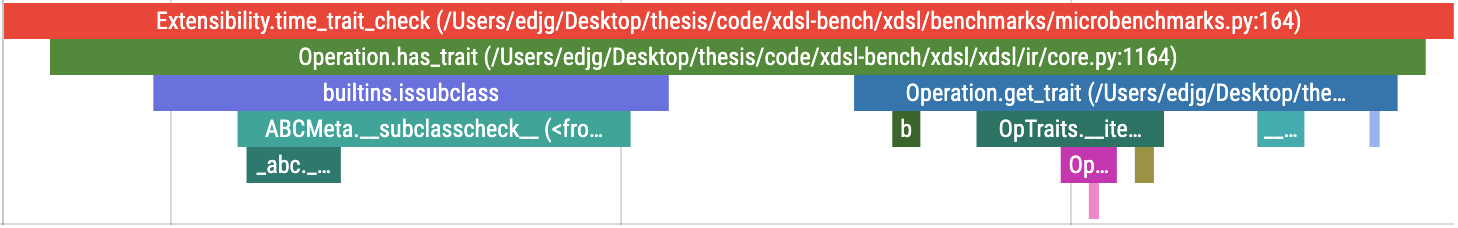
\includegraphics[width=\textwidth]{images/14_understanding_compiler_performance/trait_checks/hastrait_xdsl_viztracer.png}
        \caption{Checking for \mintinline{python}{UnregisteredOp}s constitutes around half of \mintinline{python}{has_trait}s runtime.}
        \label{fig:ubenchmark-hastrait-xdsl-viztracer}
    \end{subfigure}
    \begin{subfigure}[b]{\textwidth}
        \centering
        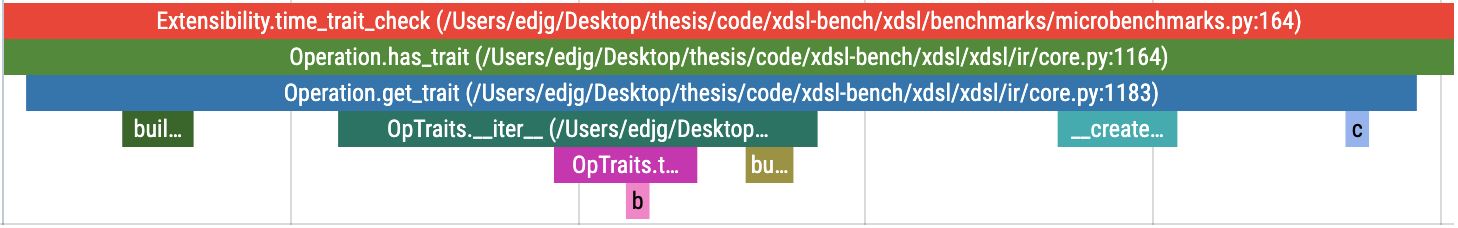
\includegraphics[width=\textwidth]{images/14_understanding_compiler_performance/trait_checks/gettrait_xdsl_viztracer.png}
        \caption{\mintinline{python}{isinstance} checks, \mintinline{python}{cast}ing and constructing iterators constitutes around half of \mintinline{python}{get_trait}s runtime.}
        \label{fig:ubenchmark-gettrait-xdsl-viztracer}
    \end{subfigure}
    \caption{\texttt{viztracer} trace of xDSL's \mintinline{python}{has_trait} and \mintinline{python}{get_trait} methods.}
    \label{fig:ubenchmark-hasgettrait-xdsl-viztracer}
\end{figure}

% Hook
By modifying xDSL's implementation to elide the extraneous code identified in the above traces (Listing \ref{listing:ubenchmark-trait-checks-both-xdsl}), we can improve its performance by a factor of eight (\autoref{tab:ubenchmark-trait-checks}).
This gives a number of insights into writing performant Python code in cases where it is unsuitable to dispatch to a lower level languages.
% Argument
Firstly, even atomic operations such as function invocation and selection statements are slow in comparison to the runtime of C++ code.
This is because \cite{}. This is substantiated by (Appendix)

% Function inlining manually (from three levels down to one) 

% Calling functions is slow! Inlining helps
% Code not on the hot path should be aggressively minimised
% Polymorphic APIs cost time in calling the isinstance function
% Casting is not free!
% This is further supported by bytecode profiling traces of these two implementations, included in the Appendix (\autoref{listing:bytecode-profiles-hastrait-original}, \autoref{listing:bytecode-profiles-hastrait-optimised}).
Unfortunately, these optimisation approaches are in tension with writing expressive and terse code -- which are motivating factors for using Python in the first place.
% Link

\begin{figure}[H]
    \centering
    \begin{subfigure}[b]{0.45\textwidth}
       \centering
        \begin{minted}[fontsize=\footnotesize]{python}
            has_trait = False
            for t in OP.traits._traits:
                if isinstance(t, TRAIT):
                    has_trait = True
                    break
        \end{minted}
        \footnotesize\vspace{5.5em}
        \captionsetup{name=Listing}
        \caption{xDSL's modified \mintinline{python}{has_trait} method.}
        \label{listing:ubenchmark-trait-checks-both-xdsl}
    \end{subfigure}
    \hfill
    \begin{subfigure}[b]{0.45\textwidth}
        \centering
        \begin{minted}[breakanywhere,fontsize=\footnotesize]{c++}
            template <template <typename T> class... Traits>
            inline bool hasTrait(TypeID traitID) {
                TypeID traitIDs[] = {TypeID::get<Traits>()...};
                for (unsigned i = 0, e = sizeof...(Traits); i != e; ++i)
                    if (traitIDs[i] == traitID)
                        return true;
                return false;
            }
            template <>
            inline bool hasTrait<>(TypeID traitID) {
                return false;
            }
        \end{minted}
        \captionsetup{name=Listing}
        \caption{MLIR's \mintinline{c++}{has_trait} method.}
        \label{listing:ubenchmark-trait-checks-both-mlir}
    \end{subfigure}
    \vspace{1em}
    \captionsetup{name=Listing}
    \caption{xDSL and MLIR methods searching trait arrays.}
    \label{listing:ubenchmark-trait-checks-both}
\end{figure}

% Hook
Having specialised xDSL's \mintinline{python}{has_trait} method to the most minimal implementation which expresses the desired functionality, we can draw comparisons between equivalent algorithms which predominantly measure the effect of the language runtime.
% Argument
Both implementations (Listing \ref{listing:ubenchmark-trait-checks-both}) share the same underlying algorithm: iteration over an operations traits, checking against each one. However, the mechanism used for this algorithm differs significantly between xDSL and MLIR.
By leveraging Python's dynamic nature, xDSL can invoke the \mintinline{python}{isinstance} function to check each trait. In contrast, MLIR uses template metaprogramming instead of the class hierarchy to define traits. This depends on \mintinline{c++}{TypeID}\footnote{\url{https://mlir.llvm.org/doxygen/TypeID_8h_source.html}}, a custom data structure to encode dynamic run-time type information in C++.
This
However, this implementation incurs complexity in its implementation (\autoref{fig:ubenchmark-hastrait-dynamism}). Despite this, the C++ implementation 
% More about MLIRs approach to dynamism
% Link

% Further examining xDSL's implementation, the \mintinline{python}{get_trait} method (\autoref{listing:ubenchmark-trait-checks-both-xdsl}) iterates over an operation's traits, invoking dynamic \mintinline{python}{isinstance} checks for each. This iterative approach is similar to MLIR's \mintinline{c++}{has_trait} method (\autoref{listing:ubenchmark-trait-checks-both-mlir}, \autoref{fig:ubenchmark-hastrait-xdsl-viztracer}). However, MLIR differs in implementation, using template metaprogramming instead of the class hierarchy to define traits. This relies on \mintinline{c++}{TypeID}, a custom data structure to encode dynamic run-time type information in C++. This is a concrete example of where C++ framework code dynamically depends on runtime user code. Dynamic languages such as Python with strong native support for run-time type introspection can express this functionality more succinctly with operations such as \mintinline{python}{isinstance}, motivating their use for this application.
% But come at the cost of weird invariant typing craziness which kinda undermines the point....

\begin{figure}[H]
    \centering
    \begin{subfigure}[b]{\textwidth}
        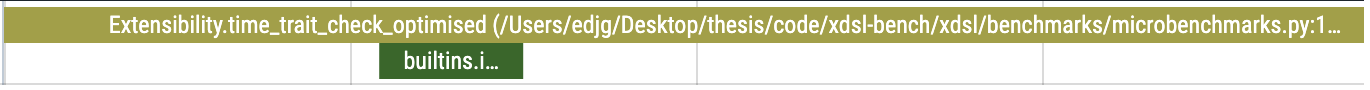
\includegraphics[width=\textwidth]{images/14_understanding_compiler_performance/trait_checks/hastrait_xdsl_viztracer_optimised.png}
        \caption{\texttt{viztracer} trace of xDSL's optimised \mintinline{python}{has_trait} implementation.}
        \label{fig:ubenchmark-hastrait-xdsl-viztracer-optimised}
    \end{subfigure}
    \begin{subfigure}[b]{\textwidth}
        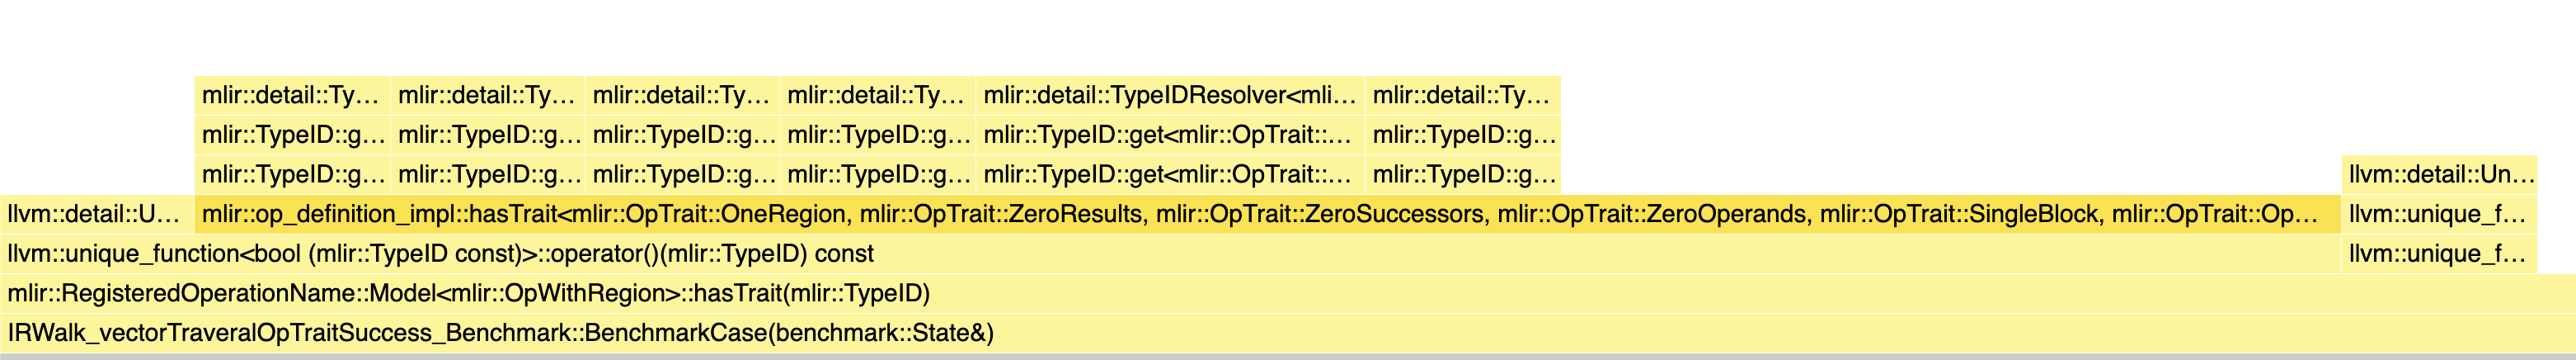
\includegraphics[width=\textwidth]{images/14_understanding_compiler_performance/trait_checks/hastrait_mlir_samply.png}
        \caption{\texttt{samply} trace of MLIR's \mintinline{c++}{has_trait} method.}
        \label{fig:ubenchmark-hastrait-mlir-samply}
    \end{subfigure}
    \caption{MLIR's dynamic trait checking using C++ RTTI is more complex than xDSL's Python implementation using \mintinline{python}{isinstance}.}
    \label{fig:ubenchmark-hastrait-dynamism}
\end{figure}


% Hook
The trait checking micro-benchmark yields two key insights.
% Argument
The first is % comparing MLIR and xDSL
The second is % quantifying the cost of dynamism and MLIRs custom implementation
% Link
However, whilst trait checking is a frequent operation, it alone is not representative of the overall performance of compiler frameworks. As such, further micro-benchmarks and examining representative workloads is required.


\subsection{Operation instantiation}
\label{ssec:op-instantiation}

% % What is the overall trend here?
% % Are we measuring the implementation of the language?
% % What does this say about dynamism?
% % What are opportunities for optimisation?


% Operations are a fundamental data structure in MLIR-like compilers. As such, their instantiation is a frequent task. Both xDSL and MLIR offer various functions to do this. The \texttt{create} functions directly construct the operation, builders offer a sugar over this construction, and cloning copies all data associated with an existing operation.

% \subsubsection{Creating operations}
% \label{sssec:ubenchmark-op-instantiation-creating}

% \subsubsection{Building operations}
% \label{sssec:ubenchmark-op-instantiation-building}

% \subsubsection{Cloning operations}
% \label{sssec:ubenchmark-op-instantiation-cloning}

% \subsubsection{Discussion}
% \label{sssec:ubenchmark-op-instantiation-discussion}

% \subsection{All microbenchmarks}
% \label{ssec:ubenchmark-all}




\section{End-to-end benchmarking}
\label{sec:e2e-benchmark}


\section{Benchmarking xDSL's pattern rewriter}
\label{sec:rewriter-benchmark}


\section{Quantifying dynamism in MLIR and xDSL}
\label{sec:quantifying-dynamism}